\begin{center}
	{\LARGE \textbf{PHYS 2240 Final Exam} }\\
	\vspace{0.5cm}
	{\Large Tuesday, May 4, 2021}
\end{center}

\vspace{1cm}
\begin{center}
	\fbox{\fbox{\parbox{5.5in}{\centering
				\textit{\large \textbf{Instructions}: You have as much time as you need to complete this exam. Take a deep breath and relax! Read each question carefully, and let me know if anything is unclear. Partial credit may be awarded, so you are encouraged to clearly and legibly show your work for each problem. Extra paper is available at the front of the room if you need it. Write your name on every extra sheet you use, and clearly label what problem you are working on. Staple this to the back of your exam when you turn it in. You may use any information contained within this exam, as well as a calculator.\\ Good luck!}}}}

\vspace{4cm}
\makebox[0.75\textwidth]{\Large \textbf{Name:}\enspace\hrulefill}
\null\vspace{2cm}
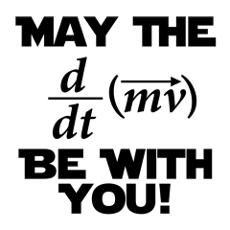
\includegraphics[width=0.3\textwidth]{cartoon2}
\end{center}